% Created by tikzDevice version 0.12.3.2 on 2022-02-15 18:25:43
% !TEX encoding = UTF-8 Unicode
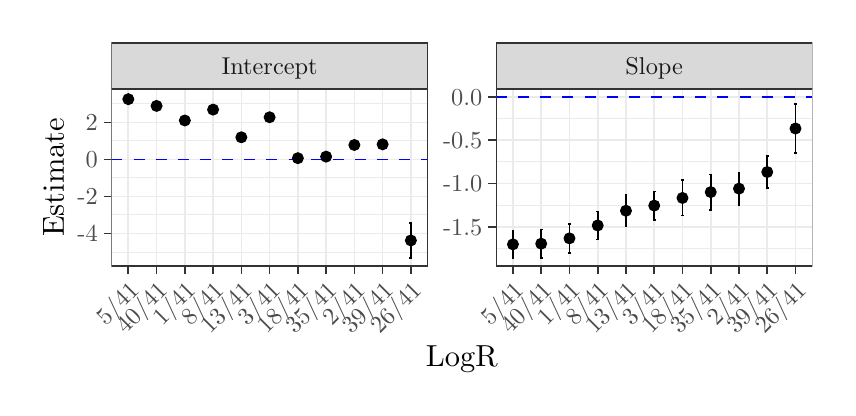
\begin{tikzpicture}[x=1pt,y=1pt]
\definecolor{fillColor}{RGB}{255,255,255}
\path[use as bounding box,fill=fillColor,fill opacity=0.00] (0,0) rectangle (289.08,130.09);
\begin{scope}
\path[clip] (  0.00,  0.00) rectangle (289.08,130.09);
\definecolor{drawColor}{RGB}{255,255,255}
\definecolor{fillColor}{RGB}{255,255,255}

\path[draw=drawColor,line width= 0.6pt,line join=round,line cap=round,fill=fillColor] (  0.00,  0.00) rectangle (289.08,130.09);
\end{scope}
\begin{scope}
\path[clip] ( 30.25, 43.96) rectangle (144.60,108.01);
\definecolor{fillColor}{RGB}{255,255,255}

\path[fill=fillColor] ( 30.25, 43.96) rectangle (144.60,108.01);
\definecolor{drawColor}{gray}{0.92}

\path[draw=drawColor,line width= 0.3pt,line join=round] ( 30.25, 49.05) --
	(144.60, 49.05);

\path[draw=drawColor,line width= 0.3pt,line join=round] ( 30.25, 62.43) --
	(144.60, 62.43);

\path[draw=drawColor,line width= 0.3pt,line join=round] ( 30.25, 75.81) --
	(144.60, 75.81);

\path[draw=drawColor,line width= 0.3pt,line join=round] ( 30.25, 89.19) --
	(144.60, 89.19);

\path[draw=drawColor,line width= 0.3pt,line join=round] ( 30.25,102.56) --
	(144.60,102.56);

\path[draw=drawColor,line width= 0.6pt,line join=round] ( 30.25, 55.74) --
	(144.60, 55.74);

\path[draw=drawColor,line width= 0.6pt,line join=round] ( 30.25, 69.12) --
	(144.60, 69.12);

\path[draw=drawColor,line width= 0.6pt,line join=round] ( 30.25, 82.50) --
	(144.60, 82.50);

\path[draw=drawColor,line width= 0.6pt,line join=round] ( 30.25, 95.88) --
	(144.60, 95.88);

\path[draw=drawColor,line width= 0.6pt,line join=round] ( 36.37, 43.96) --
	( 36.37,108.01);

\path[draw=drawColor,line width= 0.6pt,line join=round] ( 46.58, 43.96) --
	( 46.58,108.01);

\path[draw=drawColor,line width= 0.6pt,line join=round] ( 56.79, 43.96) --
	( 56.79,108.01);

\path[draw=drawColor,line width= 0.6pt,line join=round] ( 67.00, 43.96) --
	( 67.00,108.01);

\path[draw=drawColor,line width= 0.6pt,line join=round] ( 77.21, 43.96) --
	( 77.21,108.01);

\path[draw=drawColor,line width= 0.6pt,line join=round] ( 87.42, 43.96) --
	( 87.42,108.01);

\path[draw=drawColor,line width= 0.6pt,line join=round] ( 97.63, 43.96) --
	( 97.63,108.01);

\path[draw=drawColor,line width= 0.6pt,line join=round] (107.84, 43.96) --
	(107.84,108.01);

\path[draw=drawColor,line width= 0.6pt,line join=round] (118.05, 43.96) --
	(118.05,108.01);

\path[draw=drawColor,line width= 0.6pt,line join=round] (128.26, 43.96) --
	(128.26,108.01);

\path[draw=drawColor,line width= 0.6pt,line join=round] (138.47, 43.96) --
	(138.47,108.01);
\definecolor{drawColor}{RGB}{0,0,255}

\path[draw=drawColor,line width= 0.6pt,dash pattern=on 4pt off 4pt ,line join=round] ( 30.25, 82.50) -- (144.60, 82.50);
\definecolor{drawColor}{RGB}{0,0,0}
\definecolor{fillColor}{RGB}{0,0,0}

\path[draw=drawColor,line width= 0.4pt,line join=round,line cap=round,fill=fillColor] ( 56.79, 96.55) circle (  1.96);

\path[draw=drawColor,line width= 0.4pt,line join=round,line cap=round,fill=fillColor] (118.05, 87.70) circle (  1.96);

\path[draw=drawColor,line width= 0.4pt,line join=round,line cap=round,fill=fillColor] ( 87.42, 97.72) circle (  1.96);

\path[draw=drawColor,line width= 0.4pt,line join=round,line cap=round,fill=fillColor] ( 36.37,104.25) circle (  1.96);

\path[draw=drawColor,line width= 0.4pt,line join=round,line cap=round,fill=fillColor] ( 67.00,100.48) circle (  1.96);

\path[draw=drawColor,line width= 0.4pt,line join=round,line cap=round,fill=fillColor] ( 77.21, 90.48) circle (  1.96);

\path[draw=drawColor,line width= 0.4pt,line join=round,line cap=round,fill=fillColor] ( 97.63, 82.93) circle (  1.96);

\path[draw=drawColor,line width= 0.4pt,line join=round,line cap=round,fill=fillColor] (138.47, 53.20) circle (  1.96);

\path[draw=drawColor,line width= 0.4pt,line join=round,line cap=round,fill=fillColor] (107.84, 83.49) circle (  1.96);

\path[draw=drawColor,line width= 0.4pt,line join=round,line cap=round,fill=fillColor] (128.26, 87.93) circle (  1.96);

\path[draw=drawColor,line width= 0.4pt,line join=round,line cap=round,fill=fillColor] ( 46.58,101.82) circle (  1.96);

\path[draw=drawColor,line width= 0.6pt,line join=round] ( 56.28, 97.42) --
	( 57.30, 97.42);

\path[draw=drawColor,line width= 0.6pt,line join=round] ( 56.79, 97.42) --
	( 56.79, 95.68);

\path[draw=drawColor,line width= 0.6pt,line join=round] ( 56.28, 95.68) --
	( 57.30, 95.68);

\path[draw=drawColor,line width= 0.6pt,line join=round] (117.54, 88.68) --
	(118.56, 88.68);

\path[draw=drawColor,line width= 0.6pt,line join=round] (118.05, 88.68) --
	(118.05, 86.73);

\path[draw=drawColor,line width= 0.6pt,line join=round] (117.54, 86.73) --
	(118.56, 86.73);

\path[draw=drawColor,line width= 0.6pt,line join=round] ( 86.91, 99.11) --
	( 87.93, 99.11);

\path[draw=drawColor,line width= 0.6pt,line join=round] ( 87.42, 99.11) --
	( 87.42, 96.32);

\path[draw=drawColor,line width= 0.6pt,line join=round] ( 86.91, 96.32) --
	( 87.93, 96.32);

\path[draw=drawColor,line width= 0.6pt,line join=round] ( 35.86,105.10) --
	( 36.88,105.10);

\path[draw=drawColor,line width= 0.6pt,line join=round] ( 36.37,105.10) --
	( 36.37,103.40);

\path[draw=drawColor,line width= 0.6pt,line join=round] ( 35.86,103.40) --
	( 36.88,103.40);

\path[draw=drawColor,line width= 0.6pt,line join=round] ( 66.49,101.43) --
	( 67.51,101.43);

\path[draw=drawColor,line width= 0.6pt,line join=round] ( 67.00,101.43) --
	( 67.00, 99.53);

\path[draw=drawColor,line width= 0.6pt,line join=round] ( 66.49, 99.53) --
	( 67.51, 99.53);

\path[draw=drawColor,line width= 0.6pt,line join=round] ( 76.70, 91.46) --
	( 77.72, 91.46);

\path[draw=drawColor,line width= 0.6pt,line join=round] ( 77.21, 91.46) --
	( 77.21, 89.50);

\path[draw=drawColor,line width= 0.6pt,line join=round] ( 76.70, 89.50) --
	( 77.72, 89.50);

\path[draw=drawColor,line width= 0.6pt,line join=round] ( 97.12, 84.30) --
	( 98.14, 84.30);

\path[draw=drawColor,line width= 0.6pt,line join=round] ( 97.63, 84.30) --
	( 97.63, 81.56);

\path[draw=drawColor,line width= 0.6pt,line join=round] ( 97.12, 81.56) --
	( 98.14, 81.56);

\path[draw=drawColor,line width= 0.6pt,line join=round] (137.96, 59.53) --
	(138.99, 59.53);

\path[draw=drawColor,line width= 0.6pt,line join=round] (138.47, 59.53) --
	(138.47, 46.87);

\path[draw=drawColor,line width= 0.6pt,line join=round] (137.96, 46.87) --
	(138.99, 46.87);

\path[draw=drawColor,line width= 0.6pt,line join=round] (107.33, 84.82) --
	(108.35, 84.82);

\path[draw=drawColor,line width= 0.6pt,line join=round] (107.84, 84.82) --
	(107.84, 82.16);

\path[draw=drawColor,line width= 0.6pt,line join=round] (107.33, 82.16) --
	(108.35, 82.16);

\path[draw=drawColor,line width= 0.6pt,line join=round] (127.75, 89.24) --
	(128.77, 89.24);

\path[draw=drawColor,line width= 0.6pt,line join=round] (128.26, 89.24) --
	(128.26, 86.63);

\path[draw=drawColor,line width= 0.6pt,line join=round] (127.75, 86.63) --
	(128.77, 86.63);

\path[draw=drawColor,line width= 0.6pt,line join=round] ( 46.07,102.81) --
	( 47.09,102.81);

\path[draw=drawColor,line width= 0.6pt,line join=round] ( 46.58,102.81) --
	( 46.58,100.83);

\path[draw=drawColor,line width= 0.6pt,line join=round] ( 46.07,100.83) --
	( 47.09,100.83);
\definecolor{drawColor}{gray}{0.20}

\path[draw=drawColor,line width= 0.6pt,line join=round,line cap=round] ( 30.25, 43.96) rectangle (144.60,108.01);
\end{scope}
\begin{scope}
\path[clip] (169.23, 43.96) rectangle (283.58,108.01);
\definecolor{fillColor}{RGB}{255,255,255}

\path[fill=fillColor] (169.23, 43.96) rectangle (283.58,108.01);
\definecolor{drawColor}{gray}{0.92}

\path[draw=drawColor,line width= 0.3pt,line join=round] (169.23, 50.27) --
	(283.58, 50.27);

\path[draw=drawColor,line width= 0.3pt,line join=round] (169.23, 65.94) --
	(283.58, 65.94);

\path[draw=drawColor,line width= 0.3pt,line join=round] (169.23, 81.60) --
	(283.58, 81.60);

\path[draw=drawColor,line width= 0.3pt,line join=round] (169.23, 97.27) --
	(283.58, 97.27);

\path[draw=drawColor,line width= 0.6pt,line join=round] (169.23, 58.11) --
	(283.58, 58.11);

\path[draw=drawColor,line width= 0.6pt,line join=round] (169.23, 73.77) --
	(283.58, 73.77);

\path[draw=drawColor,line width= 0.6pt,line join=round] (169.23, 89.44) --
	(283.58, 89.44);

\path[draw=drawColor,line width= 0.6pt,line join=round] (169.23,105.10) --
	(283.58,105.10);

\path[draw=drawColor,line width= 0.6pt,line join=round] (175.35, 43.96) --
	(175.35,108.01);

\path[draw=drawColor,line width= 0.6pt,line join=round] (185.56, 43.96) --
	(185.56,108.01);

\path[draw=drawColor,line width= 0.6pt,line join=round] (195.77, 43.96) --
	(195.77,108.01);

\path[draw=drawColor,line width= 0.6pt,line join=round] (205.98, 43.96) --
	(205.98,108.01);

\path[draw=drawColor,line width= 0.6pt,line join=round] (216.19, 43.96) --
	(216.19,108.01);

\path[draw=drawColor,line width= 0.6pt,line join=round] (226.40, 43.96) --
	(226.40,108.01);

\path[draw=drawColor,line width= 0.6pt,line join=round] (236.61, 43.96) --
	(236.61,108.01);

\path[draw=drawColor,line width= 0.6pt,line join=round] (246.82, 43.96) --
	(246.82,108.01);

\path[draw=drawColor,line width= 0.6pt,line join=round] (257.03, 43.96) --
	(257.03,108.01);

\path[draw=drawColor,line width= 0.6pt,line join=round] (267.24, 43.96) --
	(267.24,108.01);

\path[draw=drawColor,line width= 0.6pt,line join=round] (277.45, 43.96) --
	(277.45,108.01);
\definecolor{drawColor}{RGB}{0,0,255}

\path[draw=drawColor,line width= 0.6pt,dash pattern=on 4pt off 4pt ,line join=round] (169.23,105.10) -- (283.58,105.10);
\definecolor{drawColor}{RGB}{0,0,0}
\definecolor{fillColor}{RGB}{0,0,0}

\path[draw=drawColor,line width= 0.4pt,line join=round,line cap=round,fill=fillColor] (195.77, 53.96) circle (  1.96);

\path[draw=drawColor,line width= 0.4pt,line join=round,line cap=round,fill=fillColor] (257.03, 71.93) circle (  1.96);

\path[draw=drawColor,line width= 0.4pt,line join=round,line cap=round,fill=fillColor] (226.40, 65.80) circle (  1.96);

\path[draw=drawColor,line width= 0.4pt,line join=round,line cap=round,fill=fillColor] (175.35, 51.79) circle (  1.96);

\path[draw=drawColor,line width= 0.4pt,line join=round,line cap=round,fill=fillColor] (205.98, 58.62) circle (  1.96);

\path[draw=drawColor,line width= 0.4pt,line join=round,line cap=round,fill=fillColor] (216.19, 63.94) circle (  1.96);

\path[draw=drawColor,line width= 0.4pt,line join=round,line cap=round,fill=fillColor] (236.61, 68.56) circle (  1.96);

\path[draw=drawColor,line width= 0.4pt,line join=round,line cap=round,fill=fillColor] (277.45, 93.65) circle (  1.96);

\path[draw=drawColor,line width= 0.4pt,line join=round,line cap=round,fill=fillColor] (246.82, 70.67) circle (  1.96);

\path[draw=drawColor,line width= 0.4pt,line join=round,line cap=round,fill=fillColor] (267.24, 77.93) circle (  1.96);

\path[draw=drawColor,line width= 0.4pt,line join=round,line cap=round,fill=fillColor] (185.56, 52.03) circle (  1.96);

\path[draw=drawColor,line width= 0.6pt,line join=round] (195.26, 59.21) --
	(196.28, 59.21);

\path[draw=drawColor,line width= 0.6pt,line join=round] (195.77, 59.21) --
	(195.77, 48.72);

\path[draw=drawColor,line width= 0.6pt,line join=round] (195.26, 48.72) --
	(196.28, 48.72);

\path[draw=drawColor,line width= 0.6pt,line join=round] (256.52, 77.75) --
	(257.54, 77.75);

\path[draw=drawColor,line width= 0.6pt,line join=round] (257.03, 77.75) --
	(257.03, 66.11);

\path[draw=drawColor,line width= 0.6pt,line join=round] (256.52, 66.11) --
	(257.54, 66.11);

\path[draw=drawColor,line width= 0.6pt,line join=round] (225.89, 70.94) --
	(226.91, 70.94);

\path[draw=drawColor,line width= 0.6pt,line join=round] (226.40, 70.94) --
	(226.40, 60.67);

\path[draw=drawColor,line width= 0.6pt,line join=round] (225.89, 60.67) --
	(226.91, 60.67);

\path[draw=drawColor,line width= 0.6pt,line join=round] (174.84, 56.71) --
	(175.86, 56.71);

\path[draw=drawColor,line width= 0.6pt,line join=round] (175.35, 56.71) --
	(175.35, 46.87);

\path[draw=drawColor,line width= 0.6pt,line join=round] (174.84, 46.87) --
	(175.86, 46.87);

\path[draw=drawColor,line width= 0.6pt,line join=round] (205.47, 63.65) --
	(206.49, 63.65);

\path[draw=drawColor,line width= 0.6pt,line join=round] (205.98, 63.65) --
	(205.98, 53.58);

\path[draw=drawColor,line width= 0.6pt,line join=round] (205.47, 53.58) --
	(206.49, 53.58);

\path[draw=drawColor,line width= 0.6pt,line join=round] (215.68, 69.57) --
	(216.70, 69.57);

\path[draw=drawColor,line width= 0.6pt,line join=round] (216.19, 69.57) --
	(216.19, 58.32);

\path[draw=drawColor,line width= 0.6pt,line join=round] (215.68, 58.32) --
	(216.70, 58.32);

\path[draw=drawColor,line width= 0.6pt,line join=round] (236.10, 74.94) --
	(237.12, 74.94);

\path[draw=drawColor,line width= 0.6pt,line join=round] (236.61, 74.94) --
	(236.61, 62.18);

\path[draw=drawColor,line width= 0.6pt,line join=round] (236.10, 62.18) --
	(237.12, 62.18);

\path[draw=drawColor,line width= 0.6pt,line join=round] (276.94,102.41) --
	(277.96,102.41);

\path[draw=drawColor,line width= 0.6pt,line join=round] (277.45,102.41) --
	(277.45, 84.90);

\path[draw=drawColor,line width= 0.6pt,line join=round] (276.94, 84.90) --
	(277.96, 84.90);

\path[draw=drawColor,line width= 0.6pt,line join=round] (246.31, 77.05) --
	(247.33, 77.05);

\path[draw=drawColor,line width= 0.6pt,line join=round] (246.82, 77.05) --
	(246.82, 64.29);

\path[draw=drawColor,line width= 0.6pt,line join=round] (246.31, 64.29) --
	(247.33, 64.29);

\path[draw=drawColor,line width= 0.6pt,line join=round] (266.73, 83.75) --
	(267.75, 83.75);

\path[draw=drawColor,line width= 0.6pt,line join=round] (267.24, 83.75) --
	(267.24, 72.10);

\path[draw=drawColor,line width= 0.6pt,line join=round] (266.73, 72.10) --
	(267.75, 72.10);

\path[draw=drawColor,line width= 0.6pt,line join=round] (185.05, 57.14) --
	(186.07, 57.14);

\path[draw=drawColor,line width= 0.6pt,line join=round] (185.56, 57.14) --
	(185.56, 46.93);

\path[draw=drawColor,line width= 0.6pt,line join=round] (185.05, 46.93) --
	(186.07, 46.93);
\definecolor{drawColor}{gray}{0.20}

\path[draw=drawColor,line width= 0.6pt,line join=round,line cap=round] (169.23, 43.96) rectangle (283.58,108.01);
\end{scope}
\begin{scope}
\path[clip] ( 30.25,108.01) rectangle (144.60,124.59);
\definecolor{drawColor}{gray}{0.20}
\definecolor{fillColor}{gray}{0.85}

\path[draw=drawColor,line width= 0.6pt,line join=round,line cap=round,fill=fillColor] ( 30.25,108.01) rectangle (144.60,124.59);
\definecolor{drawColor}{gray}{0.10}

\node[text=drawColor,anchor=base,inner sep=0pt, outer sep=0pt, scale=  0.88] at ( 87.42,113.27) {Intercept};
\end{scope}
\begin{scope}
\path[clip] (169.23,108.01) rectangle (283.58,124.59);
\definecolor{drawColor}{gray}{0.20}
\definecolor{fillColor}{gray}{0.85}

\path[draw=drawColor,line width= 0.6pt,line join=round,line cap=round,fill=fillColor] (169.23,108.01) rectangle (283.58,124.59);
\definecolor{drawColor}{gray}{0.10}

\node[text=drawColor,anchor=base,inner sep=0pt, outer sep=0pt, scale=  0.88] at (226.40,113.27) {Slope};
\end{scope}
\begin{scope}
\path[clip] (  0.00,  0.00) rectangle (289.08,130.09);
\definecolor{drawColor}{gray}{0.20}

\path[draw=drawColor,line width= 0.6pt,line join=round] ( 36.37, 41.21) --
	( 36.37, 43.96);

\path[draw=drawColor,line width= 0.6pt,line join=round] ( 46.58, 41.21) --
	( 46.58, 43.96);

\path[draw=drawColor,line width= 0.6pt,line join=round] ( 56.79, 41.21) --
	( 56.79, 43.96);

\path[draw=drawColor,line width= 0.6pt,line join=round] ( 67.00, 41.21) --
	( 67.00, 43.96);

\path[draw=drawColor,line width= 0.6pt,line join=round] ( 77.21, 41.21) --
	( 77.21, 43.96);

\path[draw=drawColor,line width= 0.6pt,line join=round] ( 87.42, 41.21) --
	( 87.42, 43.96);

\path[draw=drawColor,line width= 0.6pt,line join=round] ( 97.63, 41.21) --
	( 97.63, 43.96);

\path[draw=drawColor,line width= 0.6pt,line join=round] (107.84, 41.21) --
	(107.84, 43.96);

\path[draw=drawColor,line width= 0.6pt,line join=round] (118.05, 41.21) --
	(118.05, 43.96);

\path[draw=drawColor,line width= 0.6pt,line join=round] (128.26, 41.21) --
	(128.26, 43.96);

\path[draw=drawColor,line width= 0.6pt,line join=round] (138.47, 41.21) --
	(138.47, 43.96);
\end{scope}
\begin{scope}
\path[clip] (  0.00,  0.00) rectangle (289.08,130.09);
\definecolor{drawColor}{gray}{0.30}

\node[text=drawColor,rotate= 45.00,anchor=base east,inner sep=0pt, outer sep=0pt, scale=  0.88] at ( 40.66, 34.73) {5/41};

\node[text=drawColor,rotate= 45.00,anchor=base east,inner sep=0pt, outer sep=0pt, scale=  0.88] at ( 50.87, 34.73) {40/41};

\node[text=drawColor,rotate= 45.00,anchor=base east,inner sep=0pt, outer sep=0pt, scale=  0.88] at ( 61.08, 34.73) {1/41};

\node[text=drawColor,rotate= 45.00,anchor=base east,inner sep=0pt, outer sep=0pt, scale=  0.88] at ( 71.29, 34.73) {8/41};

\node[text=drawColor,rotate= 45.00,anchor=base east,inner sep=0pt, outer sep=0pt, scale=  0.88] at ( 81.50, 34.73) {13/41};

\node[text=drawColor,rotate= 45.00,anchor=base east,inner sep=0pt, outer sep=0pt, scale=  0.88] at ( 91.71, 34.73) {3/41};

\node[text=drawColor,rotate= 45.00,anchor=base east,inner sep=0pt, outer sep=0pt, scale=  0.88] at (101.92, 34.73) {18/41};

\node[text=drawColor,rotate= 45.00,anchor=base east,inner sep=0pt, outer sep=0pt, scale=  0.88] at (112.13, 34.73) {35/41};

\node[text=drawColor,rotate= 45.00,anchor=base east,inner sep=0pt, outer sep=0pt, scale=  0.88] at (122.34, 34.73) {2/41};

\node[text=drawColor,rotate= 45.00,anchor=base east,inner sep=0pt, outer sep=0pt, scale=  0.88] at (132.55, 34.73) {39/41};

\node[text=drawColor,rotate= 45.00,anchor=base east,inner sep=0pt, outer sep=0pt, scale=  0.88] at (142.76, 34.73) {26/41};
\end{scope}
\begin{scope}
\path[clip] (  0.00,  0.00) rectangle (289.08,130.09);
\definecolor{drawColor}{gray}{0.20}

\path[draw=drawColor,line width= 0.6pt,line join=round] (175.35, 41.21) --
	(175.35, 43.96);

\path[draw=drawColor,line width= 0.6pt,line join=round] (185.56, 41.21) --
	(185.56, 43.96);

\path[draw=drawColor,line width= 0.6pt,line join=round] (195.77, 41.21) --
	(195.77, 43.96);

\path[draw=drawColor,line width= 0.6pt,line join=round] (205.98, 41.21) --
	(205.98, 43.96);

\path[draw=drawColor,line width= 0.6pt,line join=round] (216.19, 41.21) --
	(216.19, 43.96);

\path[draw=drawColor,line width= 0.6pt,line join=round] (226.40, 41.21) --
	(226.40, 43.96);

\path[draw=drawColor,line width= 0.6pt,line join=round] (236.61, 41.21) --
	(236.61, 43.96);

\path[draw=drawColor,line width= 0.6pt,line join=round] (246.82, 41.21) --
	(246.82, 43.96);

\path[draw=drawColor,line width= 0.6pt,line join=round] (257.03, 41.21) --
	(257.03, 43.96);

\path[draw=drawColor,line width= 0.6pt,line join=round] (267.24, 41.21) --
	(267.24, 43.96);

\path[draw=drawColor,line width= 0.6pt,line join=round] (277.45, 41.21) --
	(277.45, 43.96);
\end{scope}
\begin{scope}
\path[clip] (  0.00,  0.00) rectangle (289.08,130.09);
\definecolor{drawColor}{gray}{0.30}

\node[text=drawColor,rotate= 45.00,anchor=base east,inner sep=0pt, outer sep=0pt, scale=  0.88] at (179.64, 34.73) {5/41};

\node[text=drawColor,rotate= 45.00,anchor=base east,inner sep=0pt, outer sep=0pt, scale=  0.88] at (189.85, 34.73) {40/41};

\node[text=drawColor,rotate= 45.00,anchor=base east,inner sep=0pt, outer sep=0pt, scale=  0.88] at (200.06, 34.73) {1/41};

\node[text=drawColor,rotate= 45.00,anchor=base east,inner sep=0pt, outer sep=0pt, scale=  0.88] at (210.27, 34.73) {8/41};

\node[text=drawColor,rotate= 45.00,anchor=base east,inner sep=0pt, outer sep=0pt, scale=  0.88] at (220.48, 34.73) {13/41};

\node[text=drawColor,rotate= 45.00,anchor=base east,inner sep=0pt, outer sep=0pt, scale=  0.88] at (230.69, 34.73) {3/41};

\node[text=drawColor,rotate= 45.00,anchor=base east,inner sep=0pt, outer sep=0pt, scale=  0.88] at (240.90, 34.73) {18/41};

\node[text=drawColor,rotate= 45.00,anchor=base east,inner sep=0pt, outer sep=0pt, scale=  0.88] at (251.11, 34.73) {35/41};

\node[text=drawColor,rotate= 45.00,anchor=base east,inner sep=0pt, outer sep=0pt, scale=  0.88] at (261.32, 34.73) {2/41};

\node[text=drawColor,rotate= 45.00,anchor=base east,inner sep=0pt, outer sep=0pt, scale=  0.88] at (271.53, 34.73) {39/41};

\node[text=drawColor,rotate= 45.00,anchor=base east,inner sep=0pt, outer sep=0pt, scale=  0.88] at (281.74, 34.73) {26/41};
\end{scope}
\begin{scope}
\path[clip] (  0.00,  0.00) rectangle (289.08,130.09);
\definecolor{drawColor}{gray}{0.30}

\node[text=drawColor,anchor=base east,inner sep=0pt, outer sep=0pt, scale=  0.88] at (164.28, 55.08) {-1.5};

\node[text=drawColor,anchor=base east,inner sep=0pt, outer sep=0pt, scale=  0.88] at (164.28, 70.74) {-1.0};

\node[text=drawColor,anchor=base east,inner sep=0pt, outer sep=0pt, scale=  0.88] at (164.28, 86.41) {-0.5};

\node[text=drawColor,anchor=base east,inner sep=0pt, outer sep=0pt, scale=  0.88] at (164.28,102.07) {0.0};
\end{scope}
\begin{scope}
\path[clip] (  0.00,  0.00) rectangle (289.08,130.09);
\definecolor{drawColor}{gray}{0.20}

\path[draw=drawColor,line width= 0.6pt,line join=round] (166.48, 58.11) --
	(169.23, 58.11);

\path[draw=drawColor,line width= 0.6pt,line join=round] (166.48, 73.77) --
	(169.23, 73.77);

\path[draw=drawColor,line width= 0.6pt,line join=round] (166.48, 89.44) --
	(169.23, 89.44);

\path[draw=drawColor,line width= 0.6pt,line join=round] (166.48,105.10) --
	(169.23,105.10);
\end{scope}
\begin{scope}
\path[clip] (  0.00,  0.00) rectangle (289.08,130.09);
\definecolor{drawColor}{gray}{0.30}

\node[text=drawColor,anchor=base east,inner sep=0pt, outer sep=0pt, scale=  0.88] at ( 25.30, 52.71) {-4};

\node[text=drawColor,anchor=base east,inner sep=0pt, outer sep=0pt, scale=  0.88] at ( 25.30, 66.09) {-2};

\node[text=drawColor,anchor=base east,inner sep=0pt, outer sep=0pt, scale=  0.88] at ( 25.30, 79.47) {0};

\node[text=drawColor,anchor=base east,inner sep=0pt, outer sep=0pt, scale=  0.88] at ( 25.30, 92.85) {2};
\end{scope}
\begin{scope}
\path[clip] (  0.00,  0.00) rectangle (289.08,130.09);
\definecolor{drawColor}{gray}{0.20}

\path[draw=drawColor,line width= 0.6pt,line join=round] ( 27.50, 55.74) --
	( 30.25, 55.74);

\path[draw=drawColor,line width= 0.6pt,line join=round] ( 27.50, 69.12) --
	( 30.25, 69.12);

\path[draw=drawColor,line width= 0.6pt,line join=round] ( 27.50, 82.50) --
	( 30.25, 82.50);

\path[draw=drawColor,line width= 0.6pt,line join=round] ( 27.50, 95.88) --
	( 30.25, 95.88);
\end{scope}
\begin{scope}
\path[clip] (  0.00,  0.00) rectangle (289.08,130.09);
\definecolor{drawColor}{RGB}{0,0,0}

\node[text=drawColor,anchor=base,inner sep=0pt, outer sep=0pt, scale=  1.10] at (156.91,  7.64) {LogR};
\end{scope}
\begin{scope}
\path[clip] (  0.00,  0.00) rectangle (289.08,130.09);
\definecolor{drawColor}{RGB}{0,0,0}

\node[text=drawColor,rotate= 90.00,anchor=base,inner sep=0pt, outer sep=0pt, scale=  1.10] at ( 13.08, 75.99) {Estimate};
\end{scope}
\end{tikzpicture}
